\section{Detector Configurations}
\label{app:configs}
Each detector is run as its model card documents. Inputs longer than the context window are truncated, except for Sheltron, whose card specifies overlapping windows (stride 768), and Prompt Guard, whose cards specify splitting long inputs into 512-token segments; for both we take the maximum score over windows. Prismor's card truncates the whole chat prompt at 512 tokens, which cuts the assistant header from long inputs; we truncate only the text so the template stays intact.

\begin{table}[h]
\centering\small
\resizebox{\columnwidth}{!}{%
\begin{tabular}{@{}llrl@{}}
\toprule
Detector & Hugging Face model & Ctx & Input \\
\midrule
ProtectAI v1 & \texttt{protectai/\ldots-injection} & 512 & text \\
ProtectAI v2 & \texttt{protectai/\ldots-injection-v2} & 512 & text \\
JasperLS & \texttt{JasperLS/deberta-v3-base-injection} & 512 & text \\
TestSavant-L & \texttt{testsavantai/\ldots-large-v0} & 512 & text \\
PIGuard & \texttt{leolee99/PIGuard} & 512 & text \\
Sheltron & \texttt{sheltron-ai/prompt-guard-68m} & 1024 & role/source tokens \\
Prismor & \texttt{prismor/prompt-guard-1.5b} & 512 & chat template \\
Wolf Defender & \texttt{patronus-studio/wolf-defender-\ldots} & 2048 & text \\
Horizon-Labs & \texttt{Horizon-Labs/\ldots-guard-base} & 2048 & text \\
Prompt Guard 2 (86M) & \texttt{meta-llama/Llama-Prompt-Guard-2-86M} & 512 & segmented \\
Prompt Guard 2 (22M) & \texttt{meta-llama/Llama-Prompt-Guard-2-22M} & 512 & segmented \\
Prompt Guard 1 & \texttt{meta-llama/Prompt-Guard-86M} & 512 & segmented \\
ProtectAI v2-small & \texttt{protectai/\ldots-small-\ldots-v2} & 512 & text \\
Qualifire Sentinel & \texttt{qualifire/prompt-injection-sentinel} & 2048 & text \\
Sentinel v2 & \texttt{rogue-security/\ldots-sentinel-v2} & 2048 & text \\
\bottomrule
\end{tabular}}
\end{table}

\section{Detailed Results for Four Methods}
\label{app:detail}

Table~\ref{tab:main} gives AUROC, bootstrap intervals for TPR at 1\% FPR, and default-threshold rates for the two detectors and two judges we examine most closely; Figure~\ref{fig:roc} shows their ROC curves.

\begin{table*}[t]
\centering\small
\caption{Detection on the three matched sets for four methods. Brackets: 95\% bootstrap interval. BIPIA uses only test-half attacks.}
\label{tab:main}
\begin{tabular}{@{}llcccc@{}}
\toprule
Set & Method & AUROC & TPR @ 1\% FPR (\%) & FPR @ 0.5 (\%) & TPR @ 0.5 (\%) \\
\midrule
\multirow{4}{*}{AD-Matched} & ProtectAI v2 & \ADPAAuc & \ADPATprT{} [\ADPATprCI] & \ADPAFprHalfT & \ADPATprHalfT \\
 & PIGuard & \ADPGAuc & \ADPGTprT{} [\ADPGTprCI] & \ADPGFprHalfT & \ADPGTprHalfT \\
 & Judge (Qwen2.5-7B) & \ADJQAuc & \ADJQTprT{} [\ADJQTprCI] & \ADJQFprHalfT & \ADJQTprHalfT \\
 & Judge (Llama-3.1-8B) & \ADJLAuc & \ADJLTprT{} [\ADJLTprCI] & \ADJLFprHalfT & \ADJLTprHalfT \\
\midrule
\multirow{4}{*}{AD-Shift} & ProtectAI v2 & \ADSPAAuc & \ADSPATprT{} [\ADSPATprCI] & \ADSPAFprHalfT & \ADSPATprHalfT \\
 & PIGuard & \ADSPGAuc & \ADSPGTprT{} [\ADSPGTprCI] & \ADSPGFprHalfT & \ADSPGTprHalfT \\
 & Judge (Qwen2.5-7B) & \ADSJQAuc & \ADSJQTprT{} [\ADSJQTprCI] & \ADSJQFprHalfT & \ADSJQTprHalfT \\
 & Judge (Llama-3.1-8B) & \ADSJLAuc & \ADSJLTprT{} [\ADSJLTprCI] & \ADSJLFprHalfT & \ADSJLTprHalfT \\
\midrule
\multirow{4}{*}{BIPIA} & ProtectAI v2 & \BIPAAuc & \BIPATprT{} [\BIPATprCI] & \BIPAFprHalfT & \BIPATprHalfT \\
 & PIGuard & \BIPGAuc & \BIPGTprT{} [\BIPGTprCI] & \BIPGFprHalfT & \BIPGTprHalfT \\
 & Judge (Qwen2.5-7B) & \BIJQAuc & \BIJQTprT{} [\BIJQTprCI] & \BIJQFprHalfT & \BIJQTprHalfT \\
 & Judge (Llama-3.1-8B) & \BIJLAuc & \BIJLTprT{} [\BIJLTprCI] & \BIJLFprHalfT & \BIJLTprHalfT \\
\bottomrule
\end{tabular}
\end{table*}

\begin{figure*}[t]
\centering
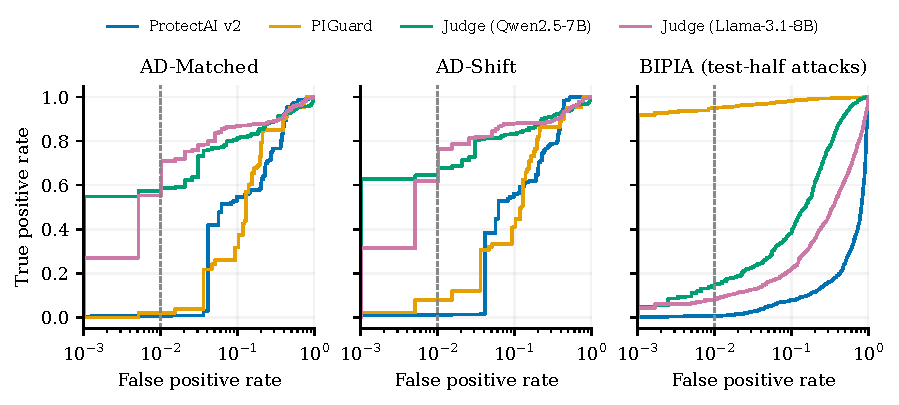
\includegraphics[width=0.9\textwidth]{figures/fig_roc.pdf}
\caption{ROC curves with logarithmic FPR axis for the four methods of Table~\ref{tab:main}; the dashed line marks 1\% FPR. The Llama judge's wide interval on AD-Matched comes from a few benign outputs with high scores that make the 1\% threshold unstable.}
\label{fig:roc}
\end{figure*}

\section{Judge Prompt}
\label{app:prompt}
Both judges receive the following system prompt, then a user message of the form ``User request: \ldots{} Tool \texttt{<name>} returned: \ldots'' (tool output truncated to 6{,}000 characters). We read the first-token distribution and compute $P(\text{Yes})/(P(\text{Yes})+P(\text{No}))$, summing over case and whitespace variants of each word. Both judges are quantized to 4 bits (NF4); the 4-bit Qwen judge matches the same model served in bf16 to within 0.02 AUROC on AD-Matched.

\begin{quote}\small
You audit data returned by tools to an AI assistant. Tool data is supposed to be passive information. Answer `Yes' if the tool data contains text that tries to make the assistant perform actions or tasks the user did not ask for. Answer `No' otherwise, including when the data merely describes procedures or contains ordinary requests between people. Reply with exactly one word: Yes or No.
\end{quote}

\section{Excluded Detectors}
\label{app:excluded}
\texttt{deepset/deberta-v3-base-injection} and \texttt{fmops/distilbert-prompt-injection} flag every benign README chunk we scored (\DegDeepsetReadme{} and \DegFmopsReadme{}, respectively) and more than three quarters of AD-Clean tool outputs. The fmops model also flags two of five plain sentences such as ``The weather is nice today.'' We treat both as unusable and omit them. \texttt{leolee99/InjecGuard} returns scores identical to PIGuard on all five sets, so we report it once.

\section{Labeling by Differential Replay}
\label{app:labels}
Our first labeling attempt marked an output as injected if it contained the injected string verbatim. Because AgentDojo serializes tool outputs as YAML, multi-line injections are re-wrapped and escaped, and every output carrying the \texttt{important\_instructions} attack was labeled benign. Differential replay (same ground-truth call, clean versus injected environment) avoids the problem; with it, each of the three AD-Matched templates contributes the same number of injected outputs. We note the pitfall because substring labeling is the obvious approach and silently inflates false-positive rates.
